\scanpage{123}
Il suffit en vertu du cor. 3 de vérifier que \deleted{$n_i=n_j$} les $n_i$ sont égaux, donc il suffit de le vérifier \inserted{$n_i=n_j$} pour \deleted{\unsure{tous les}} $Y_i,Y_j$ ``incidents''. \inserted{en prenant $Y_i=Y\cap X_i$, $Y_j=Y\cap X_j$} \deleted{Pour}

Soit $X_{ij}$ une composante irréductible de \deleted{\unsure{ceci}, soit $z$ le pt générique de} $X_i\cap X_j$ \deleted{contenant} $Z_{ij}$ et rencontrant $X_f$. \deleted{$(Z_{ij})$} on peut supposer $X=\operatorname{Spec}A_{\unsure{z}}$; \deleted{$\unsure{A}$} \deleted{donc}\inserted{avec} $D$ \deleted{\unsure{est}} de la forme $\operatorname{div}t$, où $t\in\mathbf R(A)$. Comme $D\cap X_f=0$, on a $t\in A_f^*$,

\figure{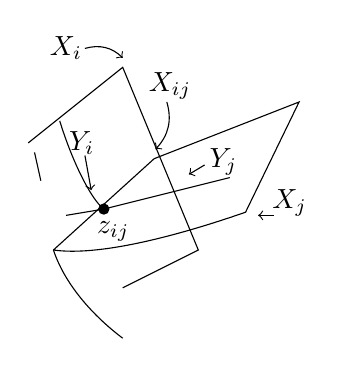
\begin{tikzpicture}[x=0.8cm,y=0.8cm]
\draw (-2,0.8)--(-0.5,2.0)--(0.7,-0.9)--(-0.5,-1.5);
\draw (-1.8,0.2)--(-1.9,0.65);
\draw (-1.6,-0.9) .. controls (-1.4,-1.5) and (-0.9,-2) .. (-0.5,-2.3);
\draw (-1.6,-0.9)--(0,0.55)--(2.3,1.45)--(1.45,-0.3) .. controls (0.3,-0.7) and (-0.9,-1.0) .. (-1.6,-0.9);
\draw (-1.4,-0.35)--(-0.8,-0.25)--(1.2,0.25);
\draw (-1.5,1.15) .. controls (-1.3,0.5) and (-1,-0.1) .. (-0.8,-0.25);
\fill (-0.8,-0.25) circle (0.09);
\node at (-0.65,-0.6) {$\unsure{z_{ij}}$};
\node at (-1.4,2.3) {$X_i$}; \draw[->] (-1.1,2.3) to[bend left] (-0.5,2.15);
\node at (0.25,1.7) {$X_{ij}$}; \draw[->] (0.2,1.45) to[bend left] (0.02,0.7);
\node at (-1.15,0.8) {$Y_i$}; \draw[->] (-1.1,0.6)--(-1,0.05);
\node at (1.1,0.5) {$Y_j$}; \draw[->] (0.8,0.45)--(0.55,0.3);
\node at (2.15,-0.15) {$X_j$}; \draw[->] (1.9,-0.35)--(1.65,-0.35);
\end{tikzpicture}}

\deleted{donc $t=x/f^m$, \inserted{$x\in A$}, Soit $A_i=(X_i)$, $f\mapsto f_i$. En se restreignant à $X_i$, on obt que
\[
t_i=\varepsilon_i f_i^{n_i},\qquad \varepsilon_i\in A_i^*,\quad \deleted{$\unsure{f_i\in K_i}$}\quad n_i\text{ un entier}.
\]
De plus, Comme $Z_{ij}\cap X_f\ne\varnothing$, $t_i|Z_{ij}$ et $t_j|Z_{ij}$}

Soit $t_i=t|X_i$, \inserted{$f_i=f|X_i$, \unsure{cor. 3}} on a
\[
t_i=\varepsilon_i f_i^{n_i}\qquad (\varepsilon_i\in A_i^*,\ n_i\in\mathbf Z).
\]
\figure{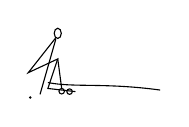
\begin{tikzpicture}[x=0.5cm,y=0.5cm]
\draw (0.2,1.6) ellipse (0.09 and 0.13);
\draw (0.16,1.5)--(-0.55,0.6)--(0.2,0.95)--(-0.05,0.2)--(0.65,0.12);
\draw (0.15,1.45)--(-0.25,0.05);\draw (0.2,0.95)--(0.3,0.2);
\draw (-0.05,0.35) .. controls (0.6,0.22) and (1.4,0.35) .. (2.8,0.16);
\draw (0.3,0.13) circle (0.07);\draw (0.5,0.12) circle (0.07);
\fill (-0.5,-0.03) circle (0.035);
\end{tikzpicture}}

\margin{\unsure{faux ici} ?\quad \fbox{\parbox{0.26\linewidth}{Attention, on ne sait pas si $X_i\times_XY=V(f_i)$ est \uuline{réduit}.}} ?}

\deleted{$Z_{ij}\in X_{ij}$}, $t_i|X_{ij}$ et $t_j|X_{ij}$ existent, et sont égaux, soit $\unsure{t'_{ij}}=\unsure{t'_{ji}}$ \unsure{on a} $=$ \uuline{\unsure{d'où}}.

\unsure{Les sections} \deleted{$t_{ij}=\varepsilon_{ij}f_i$} $f_{ij}=f|\unsure{X_{ij}|Z_{ij}}$, \inserted{$\varepsilon_{ij}=\varepsilon_i|Z_{ij}$, $\varepsilon_{ji}=\varepsilon_j|Z_{ij}$} sont des unités sur $Z_{ij}$.
\margin{122}
